% !TEX root = Entwurf_goApp.tex

\section{Client} 
	%TODO Jedes Package als subsection mit sinnvoller Bennenung und in diesen als subssubsection alle Klassen beschreiben.
	\subsection{edu.kit.sdqweb.pse.gruppe1.goApp.client.controler.service}
	Im folgenden Kapitel werden alle Services die von unserer App implementiert werden beschrieben.
	Sie alle erben von der Klasse IntentService weshalb wir zusätzlich zum Konstruktor nur eine public Methode für jeden Service implementieren und zwar die Methode onHandleIntent(Intent intent).
	Weil diese Methode bei allen unseren Services je nach Intent entscheidet, welche private Methode aufgerufen wird und sonst keine weitere Funktionalität besitzt, haben wir uns dazu entschieden im folgenden nicht für jeden Service auf die besagte Methode einzugehen sondern jeweils die Methoden zu beschreiben welche durch onHandleIntent(Intent intent) aufgerufen werden, da dies unserer Meinung nach eine bessere Definition der Services Klassen liefert und damit für bessere Verständlichkeit sorgt. 
	\subsubsection {LoginService extends IntentService}
	\subsubsection {UserService extends IntentService}
	\subsubsection {GroupService extends IntentService}
	\subsubsection {GroupSearchService extends IntentService}
	\subsubsection {RequestService extends IntentService}
	\subsubsection {RequestSearchService extends IntentService}
	\subsubsection {ParticipateService extends IntentService}
	\subsubsection {LocationService extends IntentService }
	\subsubsection {public class EventService extends IntentService}
	This Service provides methods to handle a single Event.
	\newline Methods:
	\begin{itemize}
	\item private void create(String name, Location destination, User eventAdmin, Time time)
		\begin{description}
		\item  creates an event
		\item @param name
	 	\item @param destination
	 	\item @param eventAdmin
	 	\item @param time
		\end{description}
	\item private void getEvent(Event event)
		\begin{description}
		\item gets the event from the server database
	 	\item @param event
		\end{description}
	\item public void change(Event event)
		\begin{description}
		\item
		\item @param event
		\end{description}
	\end{itemize}
	\subsubsection {GoService extends IntentService}
	\subsubsection {NotificationService extends IntentService}
	
	\subsection{edu.kit.sdqweb.pse.gruppe1.goApp.client.view}
	In diesem Abschnitt werden die Activities der goApp und ihre Interaktionen mit den Services sowie die Übergänge zu anderen Activities vorgestellt.
	Da die Activities die GUI des Benutzers bilden, werden hier ebenfalls die GUI-Ausschnitte aus dem Pflichtenheft, mit zusätzlichen Erweiterungen, den entsprechenden Activities durch welche sie dargestellt werden zugeordnet.  
	\subsubsection {LoginActivity}
	Die LoginActivity wird mit der App gestartet, hier kann sich ein Benutzer registrieren.
	\newline
	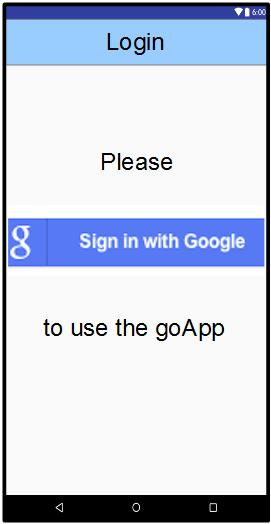
\includegraphics[width=.3\textwidth]{GUI_Login.jpg}
	\newline
	Services die von dieser Activity gestartet werden:
	\begin{itemize}
	\item LoginService
	\end{itemize}
	Von dieser Activity kann ein Benutzer zu folgenden Activities navigieren:
	\begin{itemize} 
	 \item StartActivity
	\end{itemize}
	
	\subsubsection {StartActivity}
	Die StartActivity gibt dem Benutzer eine Übersicht über alle Gruppen in denen er Mitglied ist und denen er eine Beitrittsanfrage geschickt hat.
	Außerdem kann hier der Benutzername geändert werden.
	\newline
	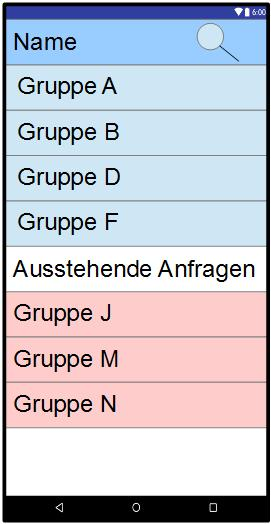
\includegraphics[width=.3\textwidth]{GUI_Start.jpg}
	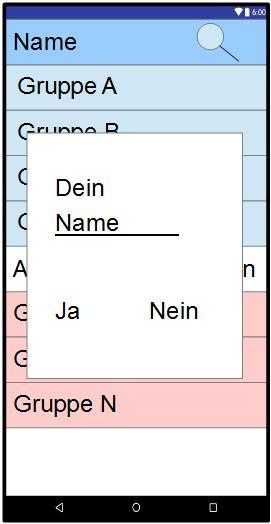
\includegraphics[width=.3\textwidth]{GUI_Start2.jpg}
	\newline
	Services die von dieser Activity gestartet werden:
	\begin{itemize}
	\item UserService
	\item GroupService
	\item GroupSearchService
	\item RequestSearchService
	\end{itemize}
	Von dieser Activity kann ein Benutzer zu folgenden Activities navigieren:
	\begin{itemize} 
	\item GroupActivity
	\item NewGroupActivity
	\end{itemize} 
	
	\subsubsection {GroupActivity}
	Die GroupActivity zeigt dem Benutzer alle anstehenden Termine einer Gruppe, bei denen er nicht abgesagt hat, an.
	\newline
	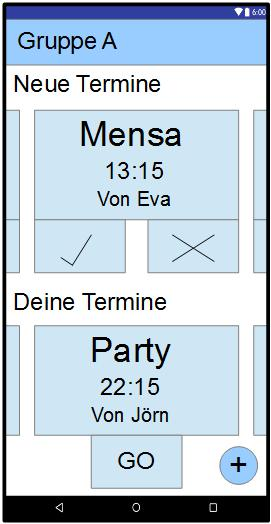
\includegraphics[width=.3\textwidth]{GUI_Group.jpg}
	\newline
	Services die von dieser Activity gestartet werden:
	\begin{itemize}
	\item EventService
	\item ParticipateService
	\item GoService
	\end{itemize}
	Von dieser Activity kann ein Benutzer zu folgenden Activities navigieren:
	\begin{itemize} 
	 \item StartActivity
	 \item GroupInfoActivity
	 \item EventActivity
	 \item NewEventActivity
	\end{itemize} 
	
	\subsubsection {GroupInfoActivity}
	Die GroupInfoActivity zeigt einem Mitglied der Gruppe deren Mitglieder an und bietet die Möglichkeit aus der Gruppe auszutreten. Der Gruppengründer sieht zusätzlich Beitrittsanfragen an die Gruppe und kann diese bearbeiten, er kann auch Mitglieder entfernen und die Gruppe löschen.
	\newline
	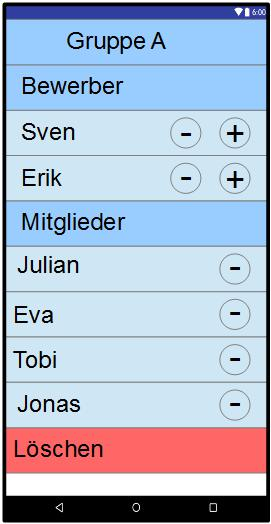
\includegraphics[width=.3\textwidth]{GUI_GruppeInfoGruender.jpg}
	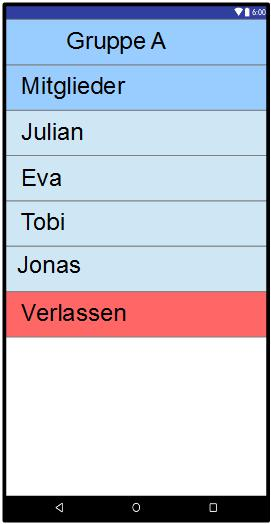
\includegraphics[width=.3\textwidth]{GUI_GruppeInfoNormal.jpg}
	\newline
	Services die von dieser Activity gestartet werden:
	\begin{itemize}
	\item GroupService
	\item RequestService
	\item RequestSearchService
	\end{itemize}
	Von dieser Activity kann ein Benutzer zu folgenden Activities navigieren:
	\begin{itemize} 
	 \item GroupActivity
	 \end{itemize}
	 
	\subsubsection {NewGroupActivity}
	Die NewGroupActivity ermöglicht es einem Benutzer nach Gruppen zu suchen um diesen Beitrittsanfragen zu schicken und neue Gruppen zu erstellen.
	\newline
	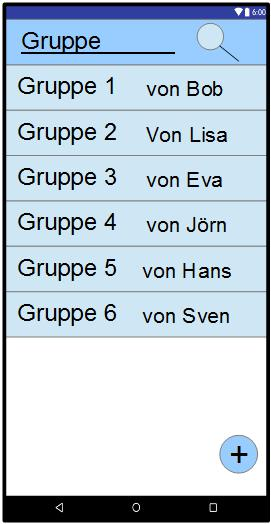
\includegraphics[width=.3\textwidth]{GUI_NeueGruppe.jpg}
	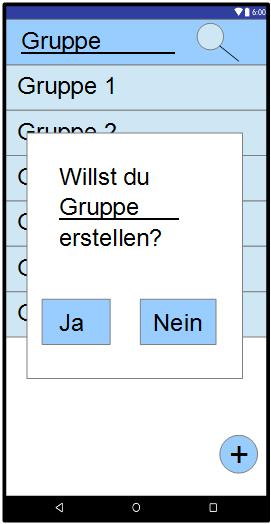
\includegraphics[width=.3\textwidth]{GUI_GruppeNeuBest.jpg}
	\newline
	Services die von dieser Activity gestartet werden:
	\begin{itemize}
	\item GroupService
	\item GroupSearchService
	\item RequestService
	\end{itemize}
	Von dieser Activity kann ein Benutzer zu folgenden Activities navigieren:
	\begin{itemize} 
	 \item StartActivity
	 \item GroupActivity
	 \end{itemize}
	 
	\subsubsection {EventActivity}
	Die EventActivity lässt einen Benutzer alle Informationen zu einem Termin einsehen und bindet eine dynamische Karte ein.
	\newline
	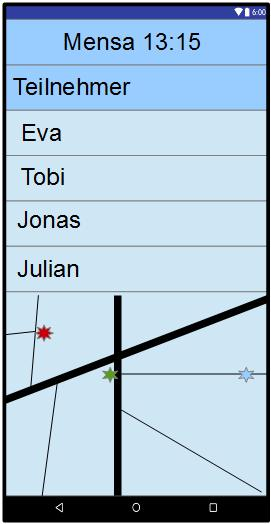
\includegraphics[width=.3\textwidth]{GUI_Termin.jpg}
	\newline
	Von dieser Activity kann ein Benutzer zu folgenden Activities navigieren:
	\begin{itemize} 
	 \item GroupActivity 
	 \end{itemize}
	 
	\subsubsection {NewEventActivity}
	Die NewEventActivity lässt einen Benutzer ein neues Event erstellen.
	\newline
	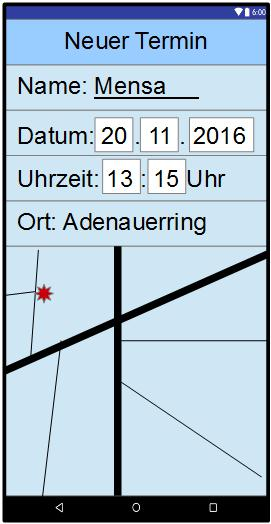
\includegraphics[width=0.3\textwidth]{GUI_NeuerTermin.jpg}
	\newline
	Services die von dieser Activity gestartet werden:
	\begin{itemize}
	\item EventService
	\end{itemize}
	Von dieser Activity kann ein Benutzer zu folgenden Activities navigieren:
	\begin{itemize} 
	 \item GroupActivity
	 \end{itemize}
	 
	
	\subsection{edu.kit.sdqweb.pse.gruppe1.goApp.client.model}
	Das Modell entspricht dem Modell des Servers (siehe Kapitel 3.1) ist aber natürlich auch auf dem Clienten zu implementieren, eine zusätzliche Beschreibung ist an dieser Stelle aber nicht nötig.
	
	\subsection{edu.kit.sdqweb.pse.gruppe1.goApp.client.controler.serverConnection}
 	Nachfolgend werden die Klassen des Paketes ServerConnection näher erläutert.
 	Dieses stellt die Schnittstelle zum Server dar. Das Paket benutzt von org.json die Klassen JSONObject und JSONArray.
 	JSONObject repräsentiert einen JSON-String, hat einen Konstruktor dem man einen JSON-String übergeben kann und besitzt die Methoden get und put um Elemente aus dem JSON-String auszulesen bzw. Elemente einem JSON-String hinzuzufügen. 
 	Ein JSONArray ist eine Menge von Objekten des gleichen Typs welche zu einem JSONObject gehören.
 	
	\subsubsection{public class HTTPConnection}
If a service wants to communicate with the server, the service has to create a HTTPConnection object and must call the sendGet/PostRequest method.
For later requests the service can use the same HTTPConnection object.
\newline Methods:
\begin{itemize}
	\item public HTTPConnection(String nameOfServlet)
		\begin{description}
		\item Constructor which expects the name of the servlet.
	 \item @param nameOfServlet The name of the servlet, the service wants to communicate with.
		\end{description}
		
		\item public void sendGetRequest(String JSON)
		\begin{description}
\item Method that handles a get request.
	 \item @param JSON The String which should be send to the server.
	 \item @return The JSONObject of the JSON-String which was sent back from the Server
		\end{description}
		
		\item public void sendPostRequest(String JSON)
		\begin{description}
\item Method that handles a post request.
	 \item @param JSON The String which should be send to the server.
	 \item @return The JSONObject of the JSON-String which was sent back from the Server
		\end{description}
	\end{itemize}
	
	\subsubsection{public enum JSONParameter}
Enumeration with all possible parameter-types for the JSON-strings.
	\newline Enum literals:
	\begin{itemize}
	
	\item ID
	\begin{description}
	\item ID of the request.
	\end{description}
	
	 \item ErrorCode
	 \begin{description}
	 \item Error code which is 0 if no error occurred.
	 \end{description}
	 
	 \item UserID
	 \begin{description}
	 \item ID of an user.
	 \end{description}
	 
     \item GroupID
     \begin{description}
	 \item ID of a group.
\end{description}

	\item EventID
	\begin{description}
	\item ID of an event.
\end{description}
	 
	\item UserName
	\begin{description}
	\item Name of an user.
\end{description}

	\item GroupName	
	\begin{description}
	\item Name of a group.
\end{description}
	 
	\item EventName
	\begin{description}
	\item Name of an event.
\end{description}
	 
	\item Method 
	\begin{description}
	\item The name of the method which should be executed on the server. For example the create method of the GroupServlet.
\end{description}
	 
	%TODO
	\item and further ones
\end{itemize}

Methods:
\begin{itemize}
	\item public String toString()
		\begin{description}
		\item Gives the corresponding name to an enum literal. Normally the enum literal name.
		\item @return The corresponding name.
		\end{description}
		
	\item public static JSONParameter fromString(String s)
		\begin{description}
		\item Gives the corresponding enum literal to a string.
	 \item @param s The string to the searched enum literal.
     \item @return The corresponding enum literal.
		\end{description}
\end{itemize}